\begin{frame}{Дополнительный слайд 2: метод роя частиц}
	\vfill
	
	\begin{columns}[T]
		
		% --- ЛЕВАЯ КОЛОНКА: МАТЕМАТИЧЕСКИЙ АППАРАТ ---
		\begin{column}{0.51\textwidth}
			\textbf{Кинематические уравнения движения:}
			\begin{tcolorbox}[
				colframe=DeepBlue!35, 
				colback=DeepBlue!1!Ivory, 
				coltext=DeepBlue, 
				boxrule=0.5pt, arc=3pt, 
				top=4pt, bottom=4pt, left=4pt, right=4pt,
				before=\vspace{3pt}, after=\vspace{0pt},
				equal height group=pso_details
				]
				\footnotesize
				Модификация вектора скорости $i$-й частицы на итерации $(k+1)$:
				{\centering $\displaystyle
					\begin{aligned}
						v_i^{(k+1)} = \omega v_i^{(k)} &+ c_1 r_1 \left( 	p_{i,\mathrm{best}} - x_i^{(k)} \right) + \\
						&+ c_2 r_2 \left( p_{\mathrm{neigh}} - x_i^{(k)} \right)
					\end{aligned}$ \par}
				
				\vspace{0.05cm}
				Коррекция положения частицы в $\mathbb{R}^4$:
				$$\mathbf{x}_i^{(k+1)} = \mathbf{x}_i^{(k)} + \mathbf{v}_i^{(k+1)}$$
				
				\vspace{0.05cm}
				• $\mathbf{x}_i, \mathbf{v}_i$ --- координаты и скорость частицы; \\
				• $\mathbf{p}_i$ --- лучший локальный вектор частицы \\
				• $\mathbf{g}$ --- наилучшее глобальное решение роя  \\
				• $r_1, r_2 \sim U(0, 1)$ --- случайные веса.
			\end{tcolorbox}
		\end{column}
		
		% --- ПРАВАЯ КОЛОНКА: СЛУЖЕБНЫЕ ПАРАМЕТРЫ ---
		\begin{column}{0.47\textwidth}
			\textbf{Параметры и ограничения численной схемы:}
			\begin{tcolorbox}[
				colframe=Burgundy!35, 
				colback=Burgundy!1!Ivory, 
				coltext=DeepBlue, 
				boxrule=0.5pt, arc=3pt, 
				top=4pt, bottom=4pt, left=4pt, right=4pt,
				before=\vspace{3pt}, after=\vspace{0pt},
				equal height group=pso_details
				]
				\footnotesize
				\textbf{Свободные параметры:}\\
				• Вес инерции: $\omega = 0.5$ \\
				• Когнитивный коэфф-т: $c_1 = 1.5$ \\
				• Социальный коэфф-т: $c_2 = 1.5$
				
				\vspace{0.2cm}
				\textbf{Параметры вычислений:}\\
				• $N = 30$ частиц \\
				• $K = 30$ итераций \\
				• $\theta \in \Omega \subset [0, 1]^4$
				
				\vspace{0.2cm}
				\textbf{Условия на границах:} \\
				При вылете частицы за пределы множества $\Omega$ применяется штраф: $\mathcal{F}(\theta) \leftarrow 10^5$.
			\end{tcolorbox}
		\end{column}
		
	\end{columns}
	
	\vspace{0.3cm}
	\scriptsize
	\textbf{Назначение этапа:} Направленный стохастический поиск в многомерных невыпуклых пространствах для гарантированного выхода из локальных экстремумов и локализации глобальной области минимума ошибки.
	\vfill
	\begin{tikzpicture}[remember picture, overlay]
		\node[opacity=0.05, inner sep=0pt] at (current page.center) 
		{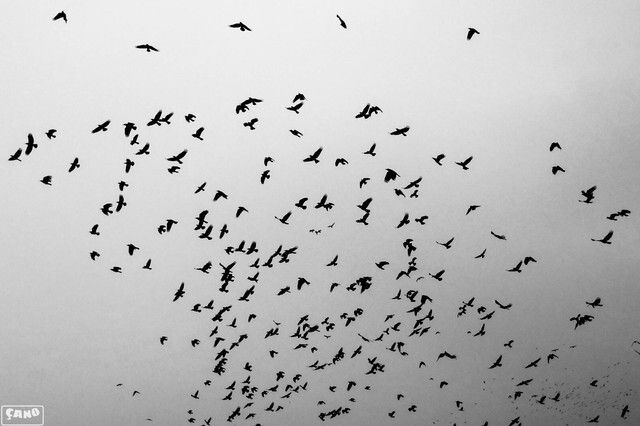
\includegraphics[width=\paperwidth, height=\paperheight, keepaspectratio]{swarm.png}}; 
	\end{tikzpicture}
\end{frame}